\documentclass{article}
\usepackage{graphicx}
\usepackage{booktabs}
\usepackage{float}
\usepackage{hyperref}
\usepackage{mathtools}
\usepackage{enumitem}
\usepackage{subcaption}
\usepackage{geometry}
 \geometry{
	left=20mm,right=20mm,%
	bindingoffset=0mm, top=20mm,bottom=20mm}

\graphicspath{ {./images/} }

\title{Investigation of the Effect of Pretraining on EEG Classification with Deep Recurrent-Convolutional Networks}
\author{Castle, Steffen \and Harbecke, David \and Rakowski, Alexander \and Stazherova, Maria}

\begin{document}
\maketitle
\pagenumbering{arabic}
	

\maketitle

\section*{Abstract}
The purpose of this research project is to investigate the use of deep neural networks in classification of EEG recordings. For this task we developed a model based on the architecture proposed by Bashivan et al. \cite{learning_eeg_repr}, with modifications for pretraining in the convolutional stage and bidirectionality in the LSTM stage. We trained and evaluated our model on a dataset consisting of EEG recordings labeled by subject. Our model showed improvement over the model proposed by Bashivan et al., with over 89\% accuracy on the task of classifying EEG recordings by subject. 

\section{Introduction}
\subparagraph{Motivation \& Background} Over the last decades, neural networks have become an extremely popular approach for the data analysis in various fields. Machine learning techniques have proven to play a crucial role in many application areas, because they possess a high classification power, are able to compute high-level abstractions of data, and provide insights into hidden relationships among the data. This is especially important in the field of neuroscience, medical signal and image processing, since the usual real-word uncertainties and incomplete information in the data set are often compounded by a poor understanding of the physical mechanisms by which the data is generated and subjective evaluation of the data by a human observer \cite{roberts}. Electroencephalography (EEG) data analysis relies a lot on statistics, and one of the challenges in modeling cognitive events from EEG data is finding representations that are invariant to inter- and intra-subject differences, therefore, machine learning methods are a crucial tool for EEG-based research. There are many clinical medical applications which include EEG-based brain-computer interface systems, or devices that are intended to change the lives of patients with disabilities, and a lot of research is being done in the area. 

Many recent studies \cite{cecotti, shamwell,driver} investigated the application of convolutional neural networks (ConvNets), which are neural networks that can learn local patterns in data by using convolutions as their key component, in the field of EEG analysis. For example, Schirrmeister et al. \cite{schirrmeister} showed how to design and train deep ConvNets with a range of different architectures to achieve the prominent results in EEG decoding tasks, by applying recent advances from the machine learning field and focusing on learning from the raw data of EEG.

Sleep analysis still remains the most unexplored area of neuroscience. Despite the fact that a lot of scientists in the field of sleep studies do not trust innovative automatic approaches, neural networks have been successfully applied to identify different sleep stages \cite{sleep} and their applications for extracting categorical cognitive sleep information are a huge focus of on-going research. Baumgart-Schmitt et al. were able to provide a reasonable agreement of the automatically generated profiles using only one EEG-channel with the profiles scored by sleep-experts on the basis of at least three EEG-channels \cite{somnology}, by applying the system SASCIA (Sleep Analysis System to Challenge Innovative Artificial Networks) to automate the sleep stage scoring. 

The state-of-the-art approach to analysing and modeling EEG during sleep recordings was presented by Bashivan et al. in the paper "Learning Representations from EEG with Deep Recurrent-Convolutional Neural Networks" \cite{learning_eeg_repr}. Bashivan et al. used a novel approach, transforming EEG data into a sequence of multi-spectral images which preserve spatial information, which, in its turn, is an important property of EEG methodology. The proposed approach showed significant improvements in accuracy of the performance on the cognitive load classification task.

\section{Data}
\subsection{Data origin \& structure}
The data set was created at a sleep laboratory \textbf{(ask:the name of the lab?)} in Canada and kindly shared with us for the purpose of this project. The researchers in the laboratory analyse and model brain activity, with the use of Electoencephalography (EEG). EEG is a noninvasive method to record electrical activity of the brain, by placing electrodes along the scalp. We received data from one experiment which was conducted in the laboratory and focused on modeling dream and sleep activity and correlating it with sleep reports. The participants were asked to come to the lab, perform a virtual tennis game, or spatial navigation task, or both and then, directly after that, to go to sleep. After a short period of time, the participants were waken up and asked to verbally describe what they dreamt about. In some session types, the full night sleeps were additionally recorded. For this particular experiment, 22-channel EEG setup was applied, with the sampling rate of 128 samples per second, and the electrodes were customized to the participants according to the International 10-20 system, as can be seen in the figure 1.
\begin{figure}[!ht]
	\centering
	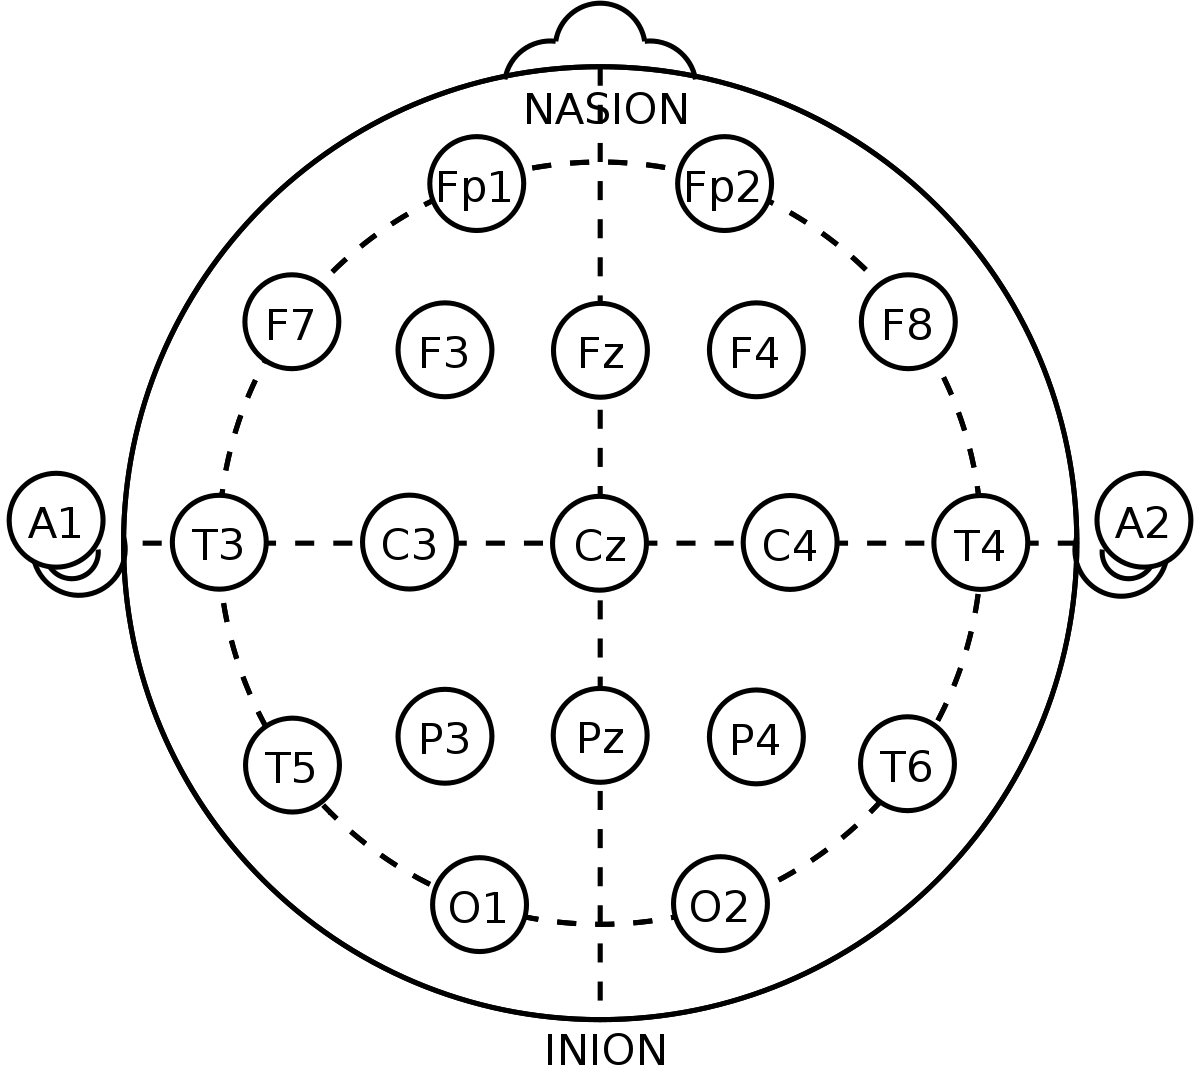
\includegraphics[scale=0.1]{eeg}
	\caption{International 10-20 EEG placement system}
\end{figure} 

All of the EEG data we received was already cleaned, so no additional filtering, or artifact rejection was needed to be performed. An example of the EEG data before preprocessing can be seen in figure 2.  For each of the 26 subjects who participated in the experiment \textbf{(look up: how many trials?)}, 3 different groups of data were provided: dream reports, mental rehearsals and verbal reports.  Dream reports contained EEG data during the short naps, mental rehearsals contained EEG data of when the participants were asked to repeat the same task they did in their minds (to think about doing the task without actually doing it). Verbal reports consisted of texts with the description of a dream provided by the participants after waking up. Each instance in the data was annotated with a label of the session type (tennis, spatial navigation, or both).
\begin{figure}[!ht]
	\centering
	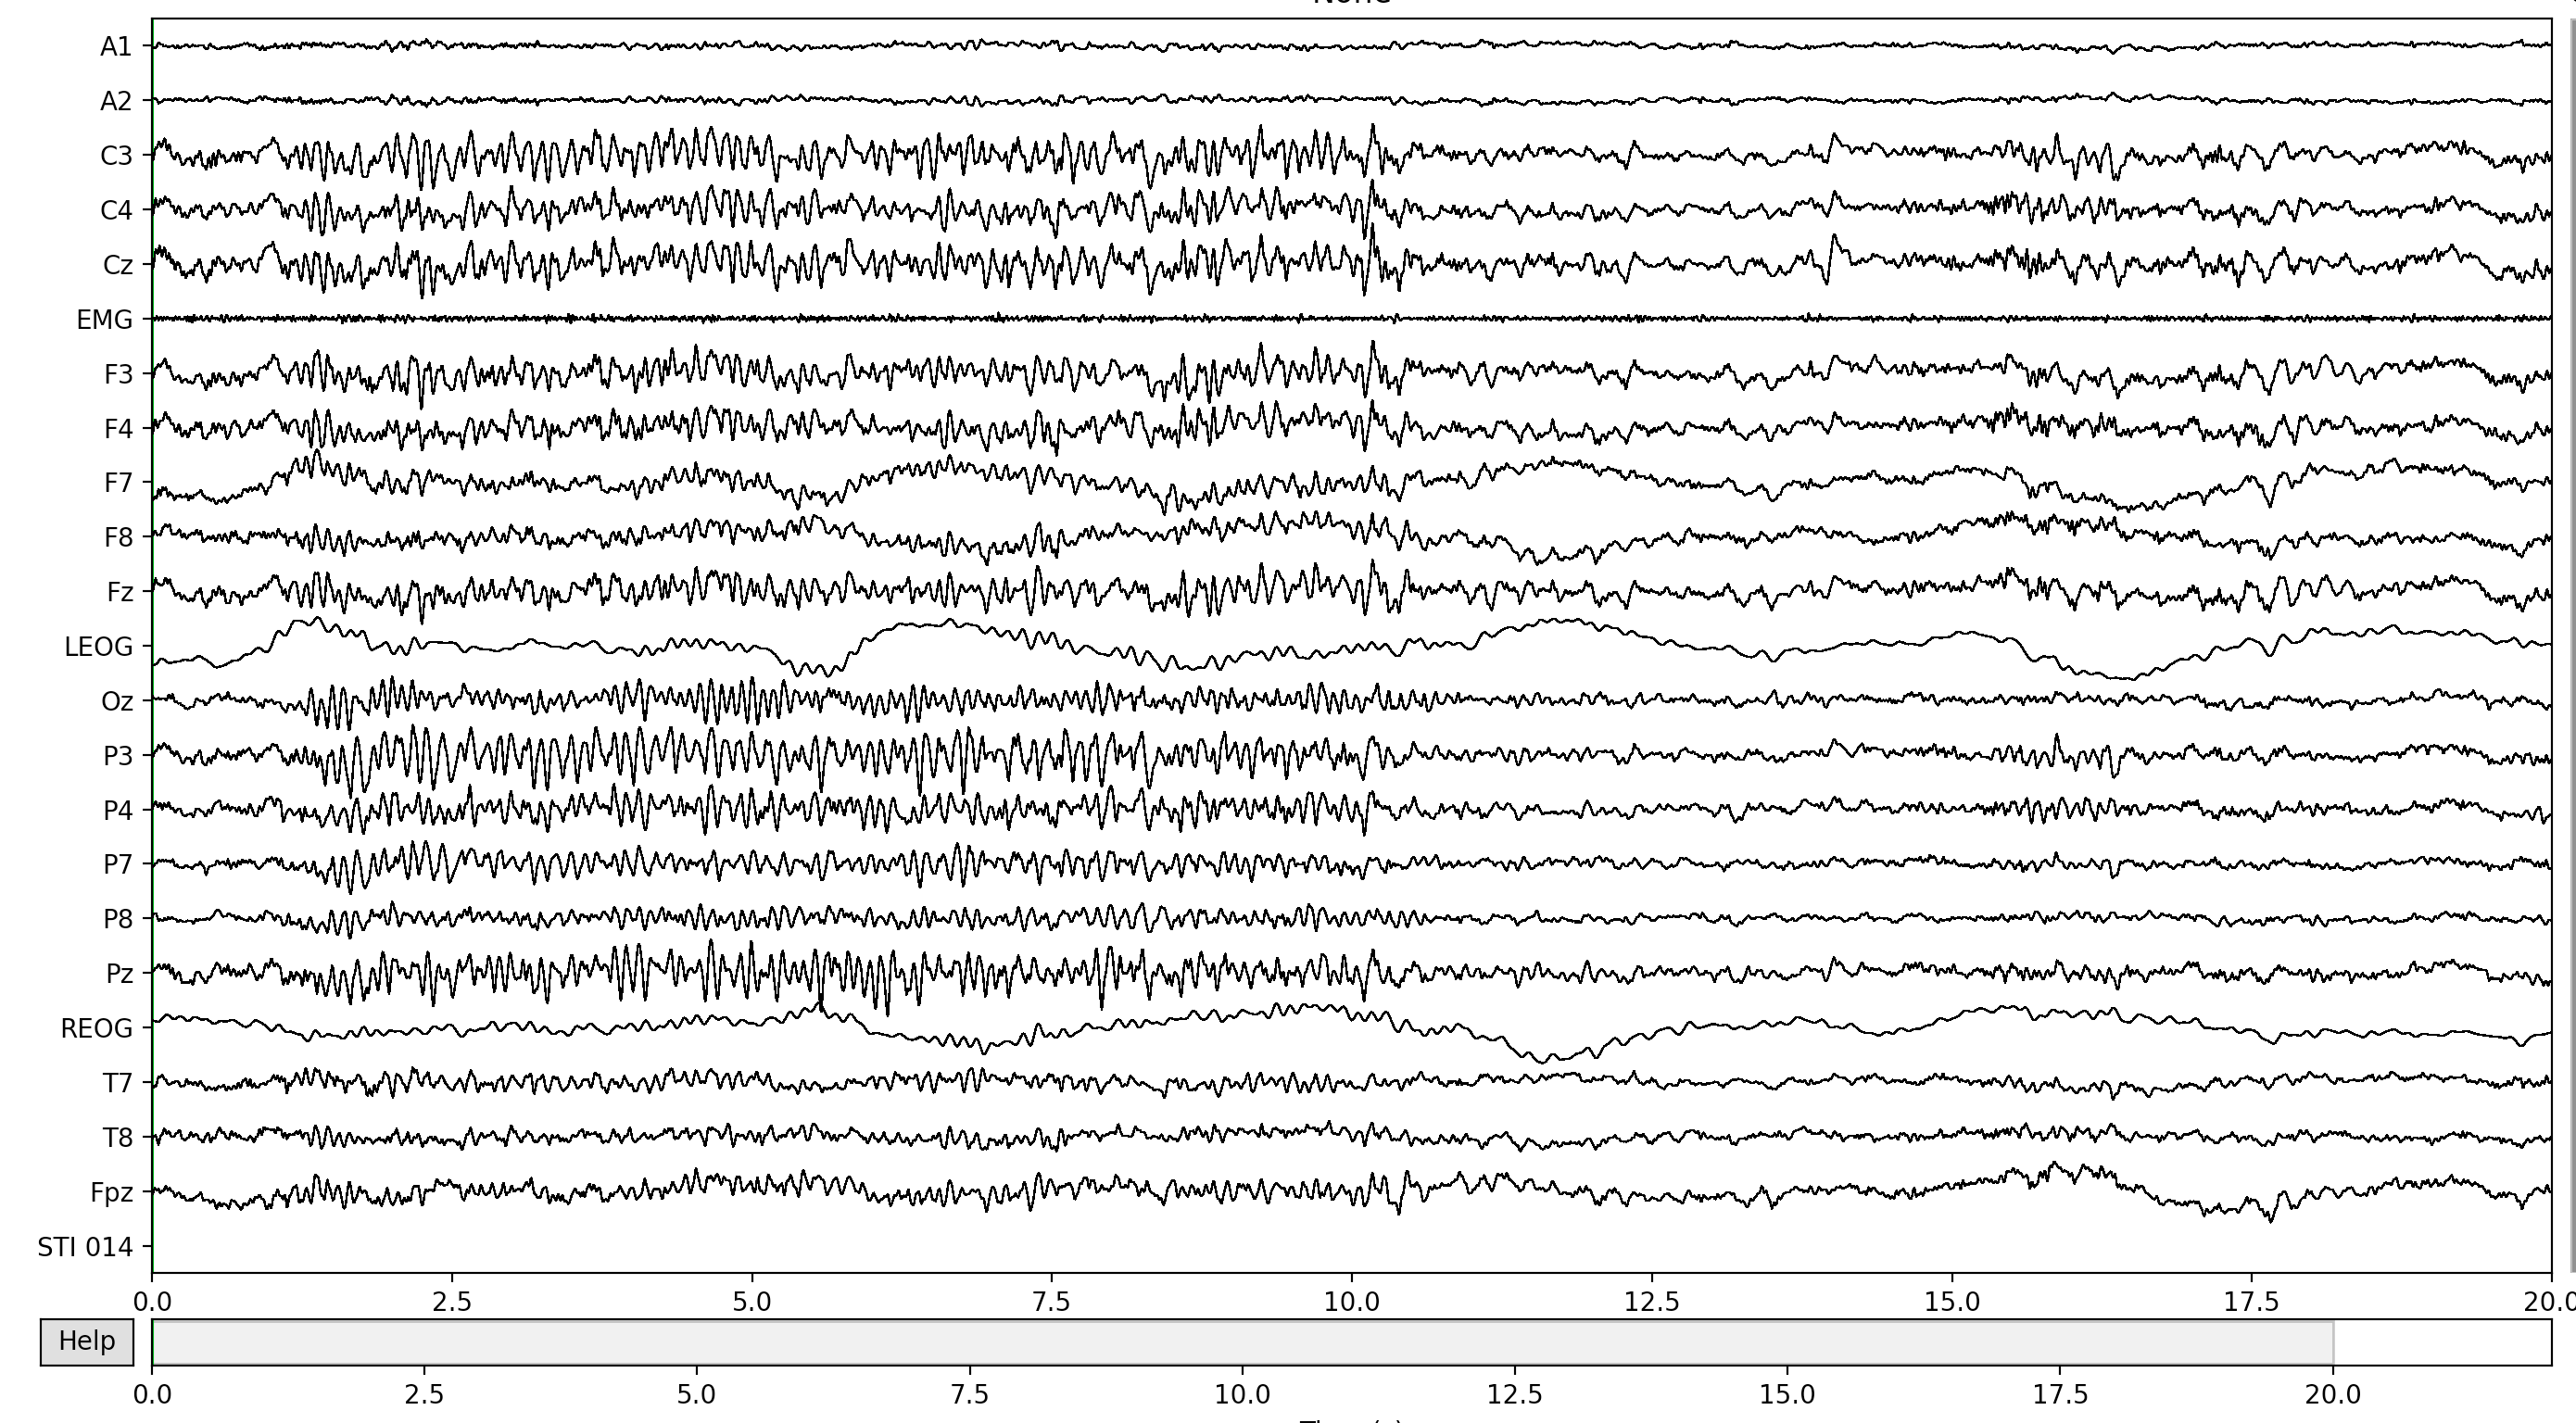
\includegraphics[scale=0.2]{eeg_ex}
	\caption{The sample of EEG data from dream reports from one of the participants. EEG traces (horizontal: time in seconds; vertical: channel locations).}
\end{figure} 

\subsection{Data Preprocessing}

\subparagraph{Motivation} EEG measurements are in form of 2-dimensional time series, indicating the change of electrode voltage over time. Such data in raw form contains noise, and has a relatively high dimensionality. Usually such data is analyzed in the frequency domain. This reduces significantly the size of the samples, and makes the influence of noise smaller. We have employed a data transformation method proposed by Bashivan et al.\cite{learning_eeg_repr}, which preserves the spatial information contained in the original data - the location of the electrodes. Measurements are aggregated over smaller periods of time, to form images of activity over the surface of the scalp. Different frequency bands are portrayed in different channels of the images. A data sample is then represented as a sequence of images. One of the motivations behind transforming the data to such a format was the fact, that there exist many Neural Network architectures successful in processing image- and video-based data. Data in visual format is also easier to analyze, what might also be helpful when investigating whether the model has learned useful features, eg. by introspection of Convolutional Filters (see Figure \ref{fig:inputs_optimized}).

\subparagraph{Implementation} Preprocessing has been done as follows:

\begin{enumerate}
 \item Raw sequences shorter than the longest one were padded with zeros.
 \item Values were then (optionally) normalized by dividing by the highest found value.
\end{enumerate}
Data was then transformed into the frequency domain. For each trial:
\begin{enumerate}[resume]
 \item Fast Fourier Transform has been applied on fixed time windows of 1 second, with 0.5 second overlap 		with the previous window.
 \item The data has then been separated into the three frequency bands - Theta (4-8 Hz), Alpha (8-13 Hz) and Beta (13-30 Hz).
 \item For each band, sum of squared values have been computed
\end{enumerate}
Finally, transformation to images has been performed. For each time window:
\begin{enumerate}[resume]
 \item In order to project the data to images, oordinates of the electrodes have been transformed from 3D into 2D space using Azimuthal Equidistant Projection, a method used for geospatial purposes \cite{snyder}.
 The motivation behind this is that the shape of the head, on which the electrodes are placed, is similar in shape to a sphere.
 \item For each band, its corresponding image has then been constructed, using the newly obtained 2D points as pixel locations. Other pixel values have been interpolated with Clough-Tocher scheme \cite{alfeld}.
 \item An RGB image has been constructed by using the bands' images as channel data.  
\end{enumerate}

\begin{figure}[h!]
 \begin{subfigure}{.5\textwidth}
   \centering
   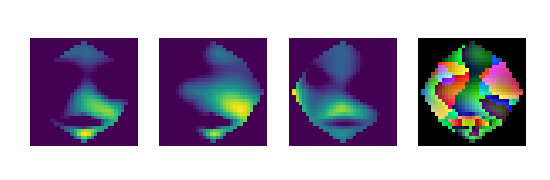
\includegraphics[width=1\linewidth]{2_cropped.png}
   \caption{}
 \end{subfigure}
 \begin{subfigure}{.5\textwidth}
   \centering
   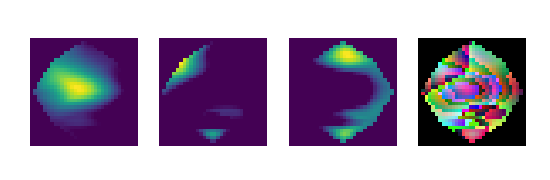
\includegraphics[width=1\linewidth]{4_cropped.png}
   \caption{}
 \end{subfigure}
 \begin{subfigure}{.5\textwidth}
   \centering
   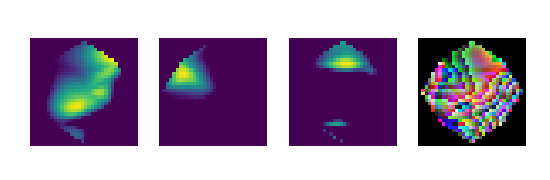
\includegraphics[width=1\linewidth]{6_cropped.png}
   \caption{}
 \end{subfigure}
 \begin{subfigure}{.5\textwidth}
   \centering
   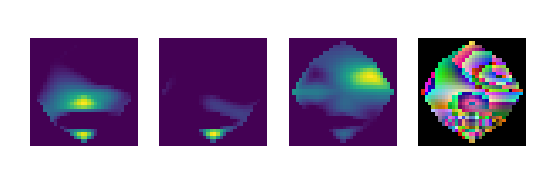
\includegraphics[width=1\linewidth]{9_cropped.png}
   \caption{}
 \end{subfigure}
 \caption{a,b,c,d - examples of the image frames of the data. First three columns show the activity in the separate frequency bands - the RGB channels of the image. The final triple channel image is shown in the fourth column.}
\end{figure}

\section{Methods}
\subsection{Baseline Methods}
Various non-deep learning methods have been employed for obtaining baseline results.
As in Bashivan et al. \cite[pp. 7-8]{learning_eeg_repr}, Support Vector Machines, Random Forest \cite{random_forests}, and sparse Logistic Regression models have been trained, using multiple parameter setting.
\subsubsection{Data Preparation}
For the baseline methods, the data has been preprocessed in a more simplified way than for the Neural Network models. This is due to the fact that the models used do not scale as well for high dimensional data, as opposed to the Convolutional Layers in the Neural Network models. Features are thus computed for the whole sequence, rather than extracting them per certain time steps. This results in data that is no more sequential in nature, but describes the whole observation.
For each of the 19 channels available in the data, Fast Fourier Transform has been applied on the whole length of a channel's data. Magnitude of each band (theta, alpha, and beta) has then been extracted and stored as the channel's features. In addition, an average over all channels has been computed. The resulting feature vector is then of size 60: \textit{(19 channels + additional averaged one) $\times$ 3 frequency bands}.
\subsubsection{Models}

\subparagraph{Support Vector Machines}
A Support Vector Machine classifier constructs a hyperplane (or set of) in the data space, which should separate the different classes. A model has been trained for each combination of the following parameters:
\begin{itemize}
	\item The penalty parameter \textbf{C} - from range of \{0.01, 0.1, 1, 10, 100\}
	\item The $\gamma$ kernel coefficient - from range of \{0.1, 0.2, .., 1, 2, .., 10\}
\end{itemize}

\subparagraph{Random Forests}
An ensemble classification method. A number of Decision Trees is being fit on different subsets of features of the training data. When classifying a data sample, the class which is given the majority of votes among the Decision Trees is chosen. A model has been trained for each of the following numbers of Decision Trees: 5, 10, 20, 50, 100, 500, 1000.

\subparagraph{Logistic Regression}
A model has been trained, using the $l_1$ as the norm for penalization, for each of the following penalization parameters \textbf{C}: \{0.01, 0.1, 1, 10, 100, 1000\}.

\section{Experiments and Results}
Our own Model consisted of the Decoder of a trained Autoencoder for the pretrained images and a Long short-Term memory\cite{LSTM} network that classifies these representations of the Decoder. \textbf{DOES ANYBODY HAVE A GRAPHIC OF OUR WHOLE ARCHITECTURE?}
\subsection{Convolutional Autoencoder}
Our approach of utilizing a convolutional autoencoder required some tuning and experimentation to find the optimal set of configurations and parameters. The first stage of tuning was to find the best activation function along with the optimal number of layers and filters, then add features such as denoising.
\subparagraph{Choosing number of layers and filters}
Bashivan et al. tested a variety of configurations for the number of layers and filters of the convolutional layers of their models. They discovered that the configuration that produced the optimal results was a set of 4 convolutions with 32 filters followed by a maxpooling layer, then a set of 2 convolutions with 64 filters followed by a maxpool, and finally one convolution with 128 filters followed by a maxpool. The size of each filter was 3x3 with a stride of 1 pixel. The activation function used was a standard ReLU. After evaluating this configuration, we found that while the autoencoder was able to reconstruct the original input EEG image with fairly good accuracy, the training time was somewhat large, and after some analysis of the filters of the convolutional layers we found that the majority were empty, or �dead� filters. 
\begin{figure}[!ht]
	\centering
    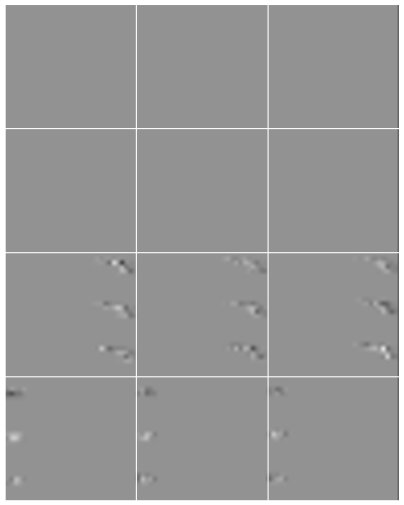
\includegraphics[scale=0.6]{inputs_orig}
    \caption{Sample of maximized inputs for individual filters in the first layer of convolutions using optimal network configuration taken from Bashivan et al. Activation maps were produced by feeding empty input (an image with values of 0 for each pixel) to the network. Inputs were then iteratively tuned using gradient ascent to find the input which maximizes the activation. Many filters appear to be mostly gray and near 0, leading to the conclusion that these filters had effectively not learned anything. A similar problem was encountered in every convolutional layer.}
\end{figure}
We opted to continue using the same filter size and stride, but test different configurations for the convolutional layer and filter numbers. In order to reduce the number of dead filters, we decided to first reduce the number of filters, and then to try some alternative activation functions specialized to combat the �dead filter� problem. After evaluating a number of different layer configurations, we found that using one layer of 32 filters, followed by one layer of 64 filters, and finally one layer of 128 filters produced the optimal results in terms of reconstructing the input. 
\subparagraph{Activation function}
\begin{figure}[!ht]
    \centering
    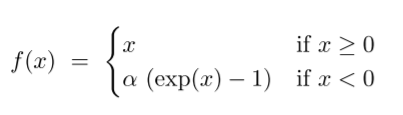
\includegraphics[scale=0.75]{elu}
    \caption{ELU activation function. The exponential function for inputs below zero allows for a gradient.}
\end{figure}
As for the activation function, after consulting the relevant literature, we decided to evaluate the performance of ELUs in lieu of the ReLU activations used in the original paper. The reasoning behind this is that dead filters may be due to the fact that the gradient of ReLU for negative inputs is zero, and thus no learning can occur for these inputs. This causes filters to �die� and simply not be updated in the training phase. In contrast, the ELU has an exponential activation value for values below zero, which allows for a gradient, and thus fewer �dead� filters. After making these modifications to the convolutional autoencoder, the number of dead filters was noticeably reduced.
\begin{figure}
    \centering
    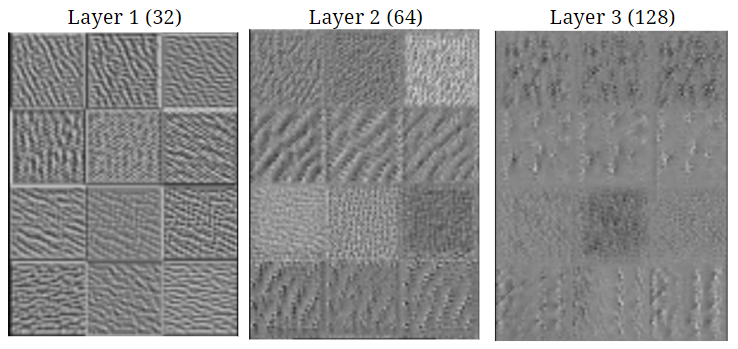
\includegraphics{inputs_optimized}
    \caption{Sample of maximized inputs for individual filters after modifications. Almost every filter now appears to have learned some representation of the input.}\label{fig:inputs_optimized}
\end{figure}
\subparagraph{Denoising}
In an attempt to add an additional level of regularization and improve generalization, we augmented our network to add denoising. In addition to the usual benefits of denoising for neural networks, we theorized that since EEG data is inherently noisy, adding a denoising component may prove especially useful in our case. As our noise component we selected simple Gaussian noise, which was added to the inputs of the autoencoder for training, with the unmodified original image as the target output. After experimenting with the variance of the noise parameter, we found that a variance of 0.0 1 provided the best reconstruction loss on the test set, although the improvement on the test set was marginal at best. 
\begin{figure}[!ht]
    \centering
    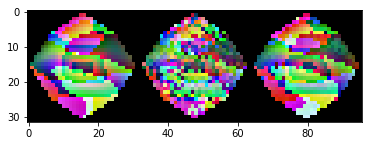
\includegraphics[scale=0.75]{denoising}
    \caption{A representation of the denoising process. Left: original image; middle: input image with additional noise (variance=0.01); right: image reconstructed by autoencoder}
\end{figure}
\subparagraph{Modified cost function}
Due to the �black� areas of the image, where the EEG activation level is 0, the autoencoder is forced to learn the useless black border of the image. This wastes training time and resources. Thus a custom cost function was implemented to remove these areas from training. A mask area was identified for the border pixels, and the cost value was set to zero for these pixels. This greatly improved training speed and accuracy.
\begin{figure}[!ht]
    \centering
    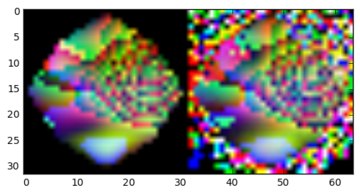
\includegraphics[scale=0.55]{mask}
    \caption{Representation of output with mask (left) vs. output after training without modified cost function (right). Even after the relevant data in the image has been encoded by the autoencoder, it is still in the process of learning the black border around the image.}
\end{figure}
\subsection{Bidirectional LSTM}
For our classification we used several layers of LSTMs, because the temporal dependencies of our data are little understood. Unidirectional and bidirectional LSTMs were tried, the latter ones learn much faster and more. Bidirectionality was implemented by simply merging the final hidden states of a normal LSTM with an LSTM with inputs reversed. Several number of layers and dropout rates were tried, $2$ layers and a $0.1$ dropout scored highest. These relatively small numbers could both be due to the small dataset. A little improvement was gained by replacing hard-sigmoid activation for the input with sigmoid activation. All models were trained for $50$ epochs over the whole training set. The models were first trained without the weights of the decoder and then compared to the model with trained decoder.
\subsection{Results}
\subsubsection{Evaluation}
Because of a very small amount of data available (766 samples in total), we have decided to use n-fold cross-validation (with \textit{n=8}) as the evaluation method. The data has been shuffled before being split into folds. For each of the $n$ runs, weights for the model with the lowest validation loss have been saved. The model's performance has then been measured on the validation fold. Final accuracy has then been computed as an average over all the runs.
Cross-validation has also been used to evaluate the baseline methods (per each method, per each configuration of parameters).
\newline
The Neural Network models have been trained on mini batches of size 32, using Adam \cite{Adam} as the optimization method.
\subsubsection{Baseline Models}
\begin{center}
\begin{tabular}{ c|c|c } 
 Model & No. parameters & Accuracy \\ 
 \hline
 SVM & - & 7.78\% $\pm 4.1\% $\\ 
 Random Forest & - & 36.72\% $\pm 7.3\%$ \\ 
 Logistic Regression & - & 33.6\% $\pm 5.8\%$ \\ 
\end{tabular}
\end{center}
\subsubsection{LSTMs without trained decoder}
\begin{center}
\begin{tabular}{ c|c|c } 
 Model & No. parameters & Accuracy \\ 
 \hline
 2 layer unidirectional LSTM & - & 18.55\% $\pm \% $\\ 
 2 layer bidirectional LSTM & - & 83.68\% $\pm \%$ \\ 
 3 layer bidirectional LSTM & - & 83.39\% $\pm \%$ \\ 
 5 layer bidirectional LSTM & - & 75.78\% $\pm \%$ \\
 2 layer bidirectional LSTM with 0.1 dropout & - & 84.08\% $\pm \%$ \\
 2 layer bidirectional LSTM with 0.2 dropout & - & 79.87\% $\pm \%$ \\
\end{tabular}
\end{center}
\subsubsection{LSTMs with trained decoder}
\begin{center}
\begin{tabular}{ c|c|c } 
 Model & No. parameters & Accuracy \\ 
 \hline
 2 layer bidirectional LSTM with 0.2 dropout & - & 89.21\% $\pm \%$ \\
\end{tabular}
\end{center}

\section{Discussion \& Conclusion}
Given the results, there is strong evidence that our modifications led to a significant improvement in classification accuracy over the model taken from Bashivan et al. It appears that the largest improvement comes from utilizing a bidirectional LSTM component, improving accuracy by over 65\%. The reason for this is most likely that context is very important in determining useful EEG segments for classification. By having access only to the forward context, unidirectional LSTMs do not have access to the future of the input sequence at each time step, thus they are less optimal at recognizing which features from the current input and hidden state are useful to pass on to the next step. It seems logical that mental processes produce exactly the type of sequences where the past and future context are equally important in determining which features are useful for classification. 

In addition, our results indicate that pretraining has led to some improvement over non-pretrained models. In the case of the 2 layer bidirectional LSTM with 0.2 dropout, adding pretraining improved classification accuracy by almost 10\%. There are probably multiple reasons for this. First of all, pretraining has long been known to be an effective form of regularization, decreasing generalization error and preventing overfitting \cite{pretraining}. But beyond this, pretraining initializes training in a different area of the problem space than without any pretraining, and this area has been shown to generally be less prone to extreme variance \cite{pretraining}. Especially for a task such as EEG classification, where the data already has a high variance due to "noise" in the recording process and in external factors such as differences between participants, mental states and possible background mental processes, the problem space probably also contains areas with high variance, which can more easily lead the training to non-optimal local minima. And beyond these properties, pretraining with a convolutional autoencoder allowed us to tune the hyperparameters of the convolutional part of our model separately from the rest of the model, rather than tuning only after training the whole model, which allowed us to more quickly choose the best parameters. 

Dropout is also known to work as a form of regularization, and given our results it appears that it also leads to an improvement in the results of the model, up to a certain point. However, too high a level of dropout degrades the performance of the model. This is probably because when the level of dropout is too high, there is not enough capacity in the model to learn the representations. 
\subsection{Further improvements}
Given the success of pretraining, it is possible that some additional pretraining would also be useful in improving accuracy. Pretraining could be added in the LSTM step as well, using the encoder from an LSTM autoencoder in place of the LSTM. And in addition to pretraining, an attention mechanism could also be added. Using attention has shown great success in previous LSTM models \cite{attention}. Instead of returning the hidden state at the end of an input sequence as is usual for LSTMs, an attention mechanism returns a learned weighted sum of all of the hidden states at each input step. This helps to preserve more of the important information in the sequence, no matter whether at the beginning or end. It is quite likely that access to this additional information would make the classification task much more effective. 

We could also gain some benefit by doing introspection, or analyzing the internal state of our trained model to see what representations it has actually learned. Bashivan et al. use a deconvolution method to look at feature maps and back projections for inputs. Using this method and working with neuroscientists familiar with brain activity patterns, we could determine the significance of what is being learned in the model and possibly use this improve our model, ie find hyperparameters that remove unrelated mental activity.
\subsection{Future investigations}
There are many directions for future work uncovered during the implementation of our project. One simple idea we could easily investigate with our model is performance on classification with different labels. Since the dataset already contains labels for mental tasks, we could easily evaluate our network to classify EEG recordings on these tasks. There is also a high amount of data available in the dataset that does not correspond to class labels, for example dream descriptions, which are simple text reports. It may be an interesting idea to investigate modifying the network to make use of this data, such as generation of text for an EEG input sequence. 
\begin{thebibliography}{99}

	\bibitem{learning_eeg_repr} 
	Bashivan  P,  Rish  I,  Yeasin  M,  Codella  N  (2016). 
	\textit{Learning  Representations from  EEG with  Deep Recurrent-Convolutional  Neural Networks}. 
	In arXiv:1511.06448 [cs]. arXiv: 1511.06448

	\bibitem{random_forests} 
	Ho, Tin Kam (1995)
	\textit{Random Decision Forests}. 
	Proceedings of the 3rd International Conference on Document Analysis and Recognition, Montreal, QC, 14�		16 August 1995. pp. 278�282

	\bibitem{snyder}
	Snyder, J.P. (1987) 
	\textit{Map Projections - A Working Manual}. 
	U.S. Geological Survey Professional Paper 1395. U.S. Govt. Print.
	Off., Washington DC
	
	\bibitem{alfeld}
	P. Alfeld (1984)
	\textit{A bivariate $C^2$ Clough-Tocher interpolant.} 
	Computer Aided Geometric Design

	\bibitem{roberts}
	Roberts S, Tarassenko L (1995).
	\textit{Automated sleep EEG analysis using an RBF network}.
	In Applications of neural networks (pp. 305-320). Springer US.

	\bibitem{schirrmeister}
	Schirrmeister R, Springenberg J, Fiederer L, Glasstetter M, Eggensperger K, Tangermann M, Ball T (2017). 
	\textit{Deep learning with convolutional neural networks for EEG decoding and visualization}.
	In Human brain mapping.

	\bibitem{sleep}
	Laengkvist M, Karlsson L, Loutfi A (2012).
	\textit{Sleep stage classification using unsupervised feature learning}.
	In Advances in Artificial Neural Systems, 2012, 5.

	\bibitem{somnology}
	Baumgart-Schmitt R, Herrmann W, Eilers R (1998). 
	\textit{On the use of neural network techniques to analyze sleep EEG data}.
	In Neuropsychobiology, 37(1), 49-58.

	\bibitem{cecotti}
	Cecotti H, Graser A (2011).
	\textit{Convolutional neural networks for P300 detection with application to brain-computer interfaces}. 
	In IEEE Trans Pattern Anal Mach Intell 33:433�445.

	\bibitem{shamwell}
	Shamwell J, Lee H, Kwon H, Marathe AR, Lawhern V, Nothwang W (2016).
	\textit{Single-trial EEG RSVP classification using convolutional neural networks}. 
	In George T, Dutta AK, Islam MS, editors. SPIE Defense+ Security, Vol. 9836. International Society for Optics and Photonics.

	\bibitem{driver}
	Hajinoroozi M, Mao Z, Jung T-P, Lin C-T, Huang Y (2016).
	\textit{EEG-based prediction of driver's cognitive performance by deep convolutional neural network}. 
	In Signal Process Image Commun 47:549�555.
	
	\bibitem{LSTM}
	Hochreiter, Sepp and Schmidhuber, J�rgen (1997).
	\textit{Long Short-term Memory}
	In Neural Computation 9:1735-80

	\bibitem{Adam}
	Kingma, D. P. \& Ba, J. (2014). 
	\textit{Adam: A Method for Stochastic Optimization.} 
	CoRR, abs/1412.6980. 
    
    \bibitem{pretraining}
    Erhan, D., Bengio, Y., Courville, A., Manzagol, P., Vincent, P., \& Bengio, S. (2010) 
    \textit{Why Does Unsupervised Pre-training Help Deep Learning?}
    Journal of Machine Learning Research 11 625-660
    
    \bibitem{attention}
    Mnih, V., Heess, N., Graves, A., \& Kavukcuoglu, K. (2014)
    \textit{Recurrent Models of Visual Attention},
    CoRR, abs/1406.6247
	
\end{thebibliography}
\end{document}

    � 2017 GitHub, Inc.
    Terms
    Privacy
    Security
    Status
    Help

    Contact GitHub
    API
    Training
    Shop
    Blog
    About

